\begin{frame}
	\begin{center}
		\Huge Engine
	\end{center}
\end{frame}


\begin{frame}
	\frametitle{Grundkonzepte}
	\begin{itemize}
		\item Oberfläche und Eingabe mit \textit{Swing}
		\item Hauptschleife
		\item Objekte
		\begin{itemize}
			\item Bild
			\item Position
			\item Beliebige Logik
		\end{itemize}
		\item Szenen
		\begin{itemize}
			\item Mehrere Objekte
			\item Beliebige Logik
		\end{itemize}
		\item Szenenstapel
		\begin{itemize}
			\item Mehrere Szenen übereinander
		\end{itemize}
		\item Sound
	\end{itemize}
\end{frame}

\begin{frame}
	\frametitle{Oberfläche}
	\begin{itemize}
		\item \textit{Java Swing Framework}
		\item Fenster
		\item Eingabe über \texttt{KeyListener} und \texttt{MouseListener}
	\end{itemize}
\end{frame}

\begin{frame}
	\frametitle{Hauptschleife}
	\begin{itemize}
		\item Endlosschleife
		\item Zähler: Um seit dem letzten Durchlauf vergangene Zeit erhöhen
		\item Erreicht $\frac{1}{60}s$: Durchlauf der Logik und Grafik
		\begin{itemize}
			\item Alle Szenen bzw. Objekte
			\item Tastaturkürzel
		\end{itemize}
	\end{itemize}
\end{frame}

\begin{frame}
	\frametitle{Objekte}
	\begin{itemize}
		\item \texttt{BaseObject}-Klasse
		\item Methoden:
		\begin{itemize}
			\item \texttt{update}
			\item \texttt{draw}
			\item \texttt{unload}
			\item \texttt{isClicked}
		\end{itemize}
	\end{itemize}
\end{frame}

\begin{frame}
	\frametitle{Szene}
	\begin{itemize}
		\item \texttt{BaseScene}-Klasse
		\item Methoden:
		\begin{itemize}
			\item \texttt{update}
			\item \texttt{draw}
			\item \texttt{unload}
		\end{itemize}
		\item Verdeckungs-Einstellungen
		\item Tags
	\end{itemize}
\end{frame}

\begin{frame}
	\frametitle{Szenenstapel}
	\begin{itemize}
		\item Liste von Szenen (\texttt{BaseScene}-Instanzen)
		\item Ausführen von \texttt{update}, \texttt{draw} und \texttt{unload}
		\item Anwenden von Verdeckungs-Einstellungen
	\end{itemize}
\end{frame}

\begin{frame}
	\frametitle{Verdeckungs-Einstellungen}
	Was soll passieren, wenn eine bestimmte Szene über einer anderen liegt?
	\vspace{0.3cm}
	
	\begin{itemize}
		\item Zuordnung Tag(s) $\rightarrow$ Regeln
		\item Werden kombiniert
		\item Soll die Szene...
		\begin{itemize}
			\item[] ... gezeichnet werden?
			\item[] ... ihre Logik ausführen?
			\item[] ... ihren Ton abspielen?
		\end{itemize}
	\end{itemize}
\end{frame}

\begin{frame}
	\begin{center}
		\begin{figure}
			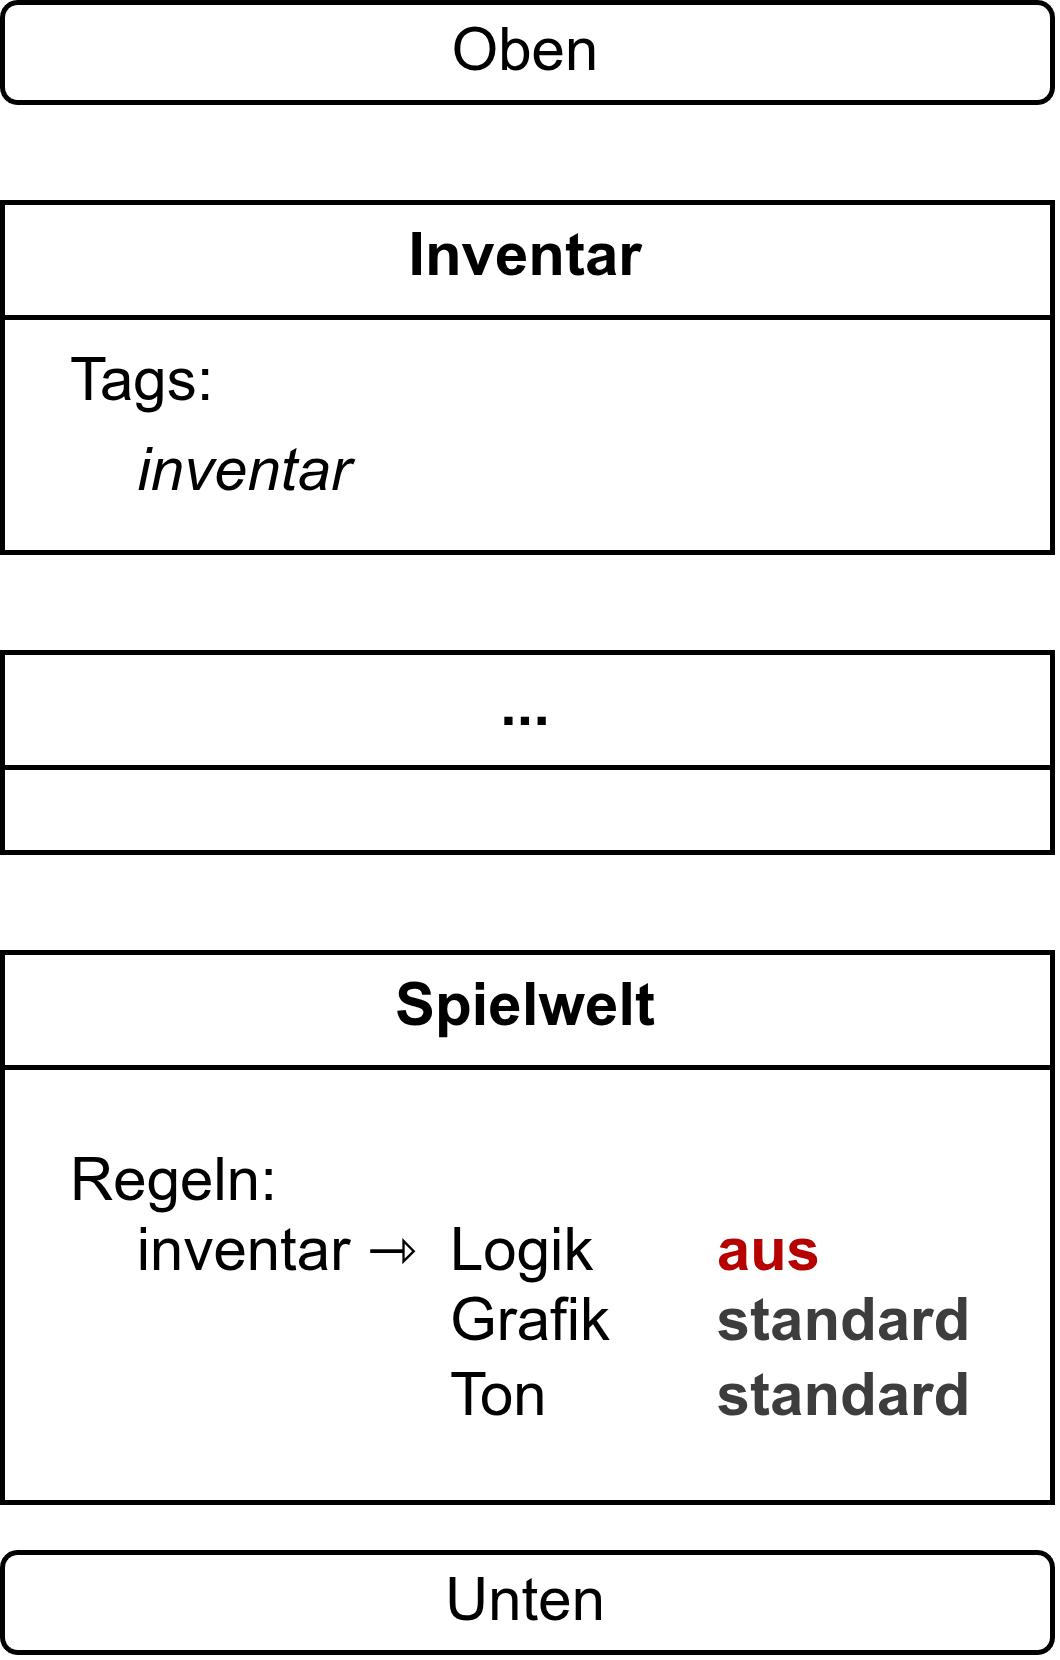
\includegraphics[width=0.4\textwidth]{bilder/Verdecken.drawio.png}
			\caption{Beispiel Verdeckungs-Einstellungen}
		\end{figure}
	\end{center}
\end{frame}

\begin{frame}
	\frametitle{Sound}
	\begin{itemize}
		\item \textit{Java Sound API}
		\item \textit{FFSampledSP} für mehr unterstzützte Formate durch \textit{ffmpeg}
		\item Wiedergabesteuerung:
		\begin{itemize}
			\item Anhalten und Fortsetzen
			\item Stoppen
			\item Endlosschleife
			\item Lautstärke
		\end{itemize}
	\end{itemize}
\end{frame}

\begin{frame}
	\frametitle{ClipSound}
	\begin{itemize}
		\item \texttt{Clip}-Klasse
		\item Gesamte Daten in den Speicher laden
		\item Einfache und schnelle Wiedergabesteuerung
	\end{itemize}
\end{frame}

\begin{frame}
	\frametitle{StreamSound}
	\begin{itemize}
		\item Stückweises Laden mit \texttt{AudioInputStream}
		\item Abspielen mit \texttt{SourceDataLine}
		\item Wiedergabe in einem separaten Thread
	\end{itemize}
\end{frame}

\begin{frame}
	\frametitle{Sound-Gruppen}
	\begin{itemize}
		\item Zusammenfassen mehrerer Sounds
		\item Gemeinsames Pausieren, Fortsetzen und Stoppen
		\item Je eine Sound-Gruppe je Szene
		\begin{itemize}
			\item Wird beim Entfernen der Szene gestoppt
		\end{itemize}
	\end{itemize}
\end{frame}